\documentclass[11pt]{article}
\usepackage{cite}
\usepackage{float}
\usepackage[a4paper,margin=2.5cm]{geometry}
\usepackage{amsmath,amssymb,graphicx}
\usepackage{graphicx}
\usepackage{hyperref}
\usepackage{amsmath,amssymb,graphicx}
\usepackage{geometry}
\geometry{a4paper, margin=1in}
\usepackage{caption}
\usepackage{booktabs}
\usepackage{tabularx}
\usepackage{authblk}
\usepackage{makeidx}
\makeindex



\title{The Spaciotemporal Vortex Model: Toward a Physically Grounded Framework for Cyclic Time and Energy Transitions}
\author{Jeremy Erich Resch}
\date{March 30, 2025}

% --- Added for improved references and glossary ---
\usepackage{cleveref}
\usepackage[acronym]{glossaries}

\makeglossaries

\newglossaryentry{entropy}
{
    name=entropy,
    description={A measure of disorder or randomness in a system.}
}

\newglossaryentry{energy}
{
    name=energy,
    description={The capacity to do work or produce change.}
}

\newglossaryentry{quantum}
{
    name=quantum,
    description={Relating to the smallest discrete quantity of some physical property.}
}

\newglossaryentry{layer}
{
    name=layer,
    description={A discrete level or slice in a structured system.}
}

\newglossaryentry{curvature}
{
    name=curvature,
    description={Measure of deviation from flat geometry.}
}

\newglossaryentry{vortex}
{
    name=vortex,
    description={A region where energy or matter spirals around an axis.}
}

\newglossaryentry{evolution}
{
    name=evolution,
    description={Gradual change or development over time.}
}

\newglossaryentry{state}
{
    name=state,
    description={The condition or configuration of a system at a given moment.}
}

\newglossaryentry{temperature}
{
    name=temperature,
    description={A measure of the average kinetic energy of particles.}
}

\newglossaryentry{collapse}
{
    name=collapse,
    description={A gravitational contraction or breakdown of structure.}
}

\newglossaryentry{transition}
{
    name=transition,
    description={Change from one state or condition to another.}
}

\newglossaryentry{geometry}
{
    name=geometry,
    description={Mathematical description of space, form, and structure.}
}




\begin{document}
\maketitle

\section*{Abstract}

The Spaciotemporal Vortex Model (SVM) offers a physically grounded framework in that time is reinterpreted as a layered fourth spatial dimension. Temporal evolution results from energy transitions between discrete temporal layers. Unlike conventional cosmological models, that treat time as a continuous linear axis and fail to address the low-entropy initial state, arrow of time, or dark phenomena, SVM introduces a novel mechanism: gravitational resistance to inter-layer transitions. This reinterpretation provides a thermodynamically coherent basis for cyclic cosmological dynamics, entropy management, and information encoding via curvature. The model derives formal evolution laws, thermodynamic couplings, and quantization paths, offering multiple empirical implications for entropy collapse, dark energy behavior, and curvature-entropy correspondence.

\section{Introduction}

Contemporary cosmological models based on General Relativity conceptualize time as a linear, continuous dimension, fundamentally distinct from space. However, they leave unresolved several foundational problems:

In the Spaciotemporal Vortex Model, time is not considered as an independent parameter but as a fourth spatial dimension composed of discrete layers. Each layer represents a distinct state of the universe, and the progression through these layers gives rise to the perception of a unidirectional flow of time.

\begin{itemize}
    \item The origin of the arrow of time,
    \item The mechanism behind the universe's extremely low initial entropy,
    \item The nature of dark matter and dark energy,
    \item The inability to naturally implement cyclic or entropy-resetting cosmologies.
\end{itemize}

The Spaciotemporal Vortex Model (SVM) introduces a restructured interpretation of ti


\subsection*{Operator Definition}
Let $f(\Delta E_n(x)) := \alpha \, \nabla^2 \Delta E_n(x)$ with $\alpha$ a dimensionless scaling factor.
The temporal layer transition becomes:

\begin{equation*}
S_{n+1}(x) = S_n(x) + \alpha \nabla^2 \Delta E_n(x)
\end{equation*}

Where $\nabla^2$ introduces spatial locality and diffusion-like behavior. 
If $[\Delta E] = \mathrm{J/m^3}$, then:

\begin{equation*}
[f(\Delta E)] = \mathrm{J/m^5}
\quad \Rightarrow \quad [S_{n+1}] = [S_n] + \mathrm{J/m^5}
\end{equation*}

\subsection*{Symbol Analysis}
\begin{tabular}{|c|l|l|c|}
\hline
Symbol & Meaning & Unit/Type & Consistent? \\
\hline
$S_n$ & State per temporal layer & Energy distribution & Yes \\
$\pi_n$ & Transition momentum & Energy per layer & Yes \\
$T_n$ & Temperature in layer & [K] & Yes \\
$Q_n$ & Heat transfer & [J] & Yes \\
\hline
\end{tabular}


\section{Quantum Thermodynamic Extension}

To extend the spaciotemporal model toward a quantum thermodynamic formalism, we promote the classical variables to operators:

\begin{equation*}
\hat{S}_n, \quad \hat{\pi}_n, \quad [\hat{S}_n, \hat{\pi}_n] = i\hbar
\end{equation*}

The discrete action becomes a quantum path sum over all possible layer evolutions:

\begin{equation*}
Z = \sum_{\text{paths}} e^{-A[S]/\hbar}
\end{equation*}

Including quantum fluctuations of entropy and temperature:

\begin{equation*}
Z = \int \mathcal{D}S\, \mathcal{D}T\, \mathcal{D}Q\, e^{- \sum_n L(S_n, T_n, Q_n)/\hbar}
\end{equation*}

This formulation allows for a quantum statistical interpretation of interlayer dynamics, where temporal evolution reflects probabilistic thermal behavior.

\section{Information Geometry}

We define a Riemannian metric over the thermodynamic layer state space $\Omega_n := \{S_n, \pi_n, T_n, Q_n\}$ using curvature of the free energy $F(S_n)$:

\begin{equation*}
g_{ab} = \partial_a \partial_b F(S_n)
\end{equation*}

In terms of statistical physics, this corresponds to:

\begin{equation*}
g_{ab} = -\partial_a \partial_b \log Z
\end{equation*}

The metric captures fluctuations and geodesic paths in the thermodynamic manifold. The curvature $R$ of this manifold may be interpreted as encoding gravitational analogues in the SVM framework.

\printglossaries

\section{Conclusion and Outlook}

The Spaciotemporal Vortex Model (SVM) provides a physically motivated and mathematically consistent alternative to conventional cosmological models by redefining time as a layered spatial dimension. This ontological shift allows energy and entropy to evolve along discrete temporal transitions, that are interpreted as physical processes rather than abstract parameters.

\subsection*{Empirical Priorities}

Key avenues for future empirical investigation include:
\begin{itemize}
    \item Detection of entropy-curvature correlations in the CMB.
    \item Searching for discrete imprints or "layer scars" in gravitational wave spectra.
    \item Investigating temperature fluctuations tied to quantum entropy effects.
\end{itemize}

\subsection*{Computational Tasks}

We aim to simulate:
\begin{itemize}
    \item Layered state evolutions using finite-difference or finite-element methods.
    \item Entropy dispersion as geometric diffusion in $\Omega_n$.
    \item Free energy landscapes and curvature-induced state changes.
\end{itemize}

\subsection*{Theoretical Development}

Future refinements of the model will involve:
\begin{itemize}
    \item Tensorial formulations of $g_{ab}$ with curvature invariants.
    \item Deriving gravitational field equations based on thermodynamic conjugates.
    \item Incorporating black hole boundary layers as entropy flux gates.
\end{itemize}

SVM proposes a coherent language that bridges thermodynamic irreversibility,


\section{Visualization of Layer Dynamics}

\begin{figure}[!htbp]
\centering
\centering
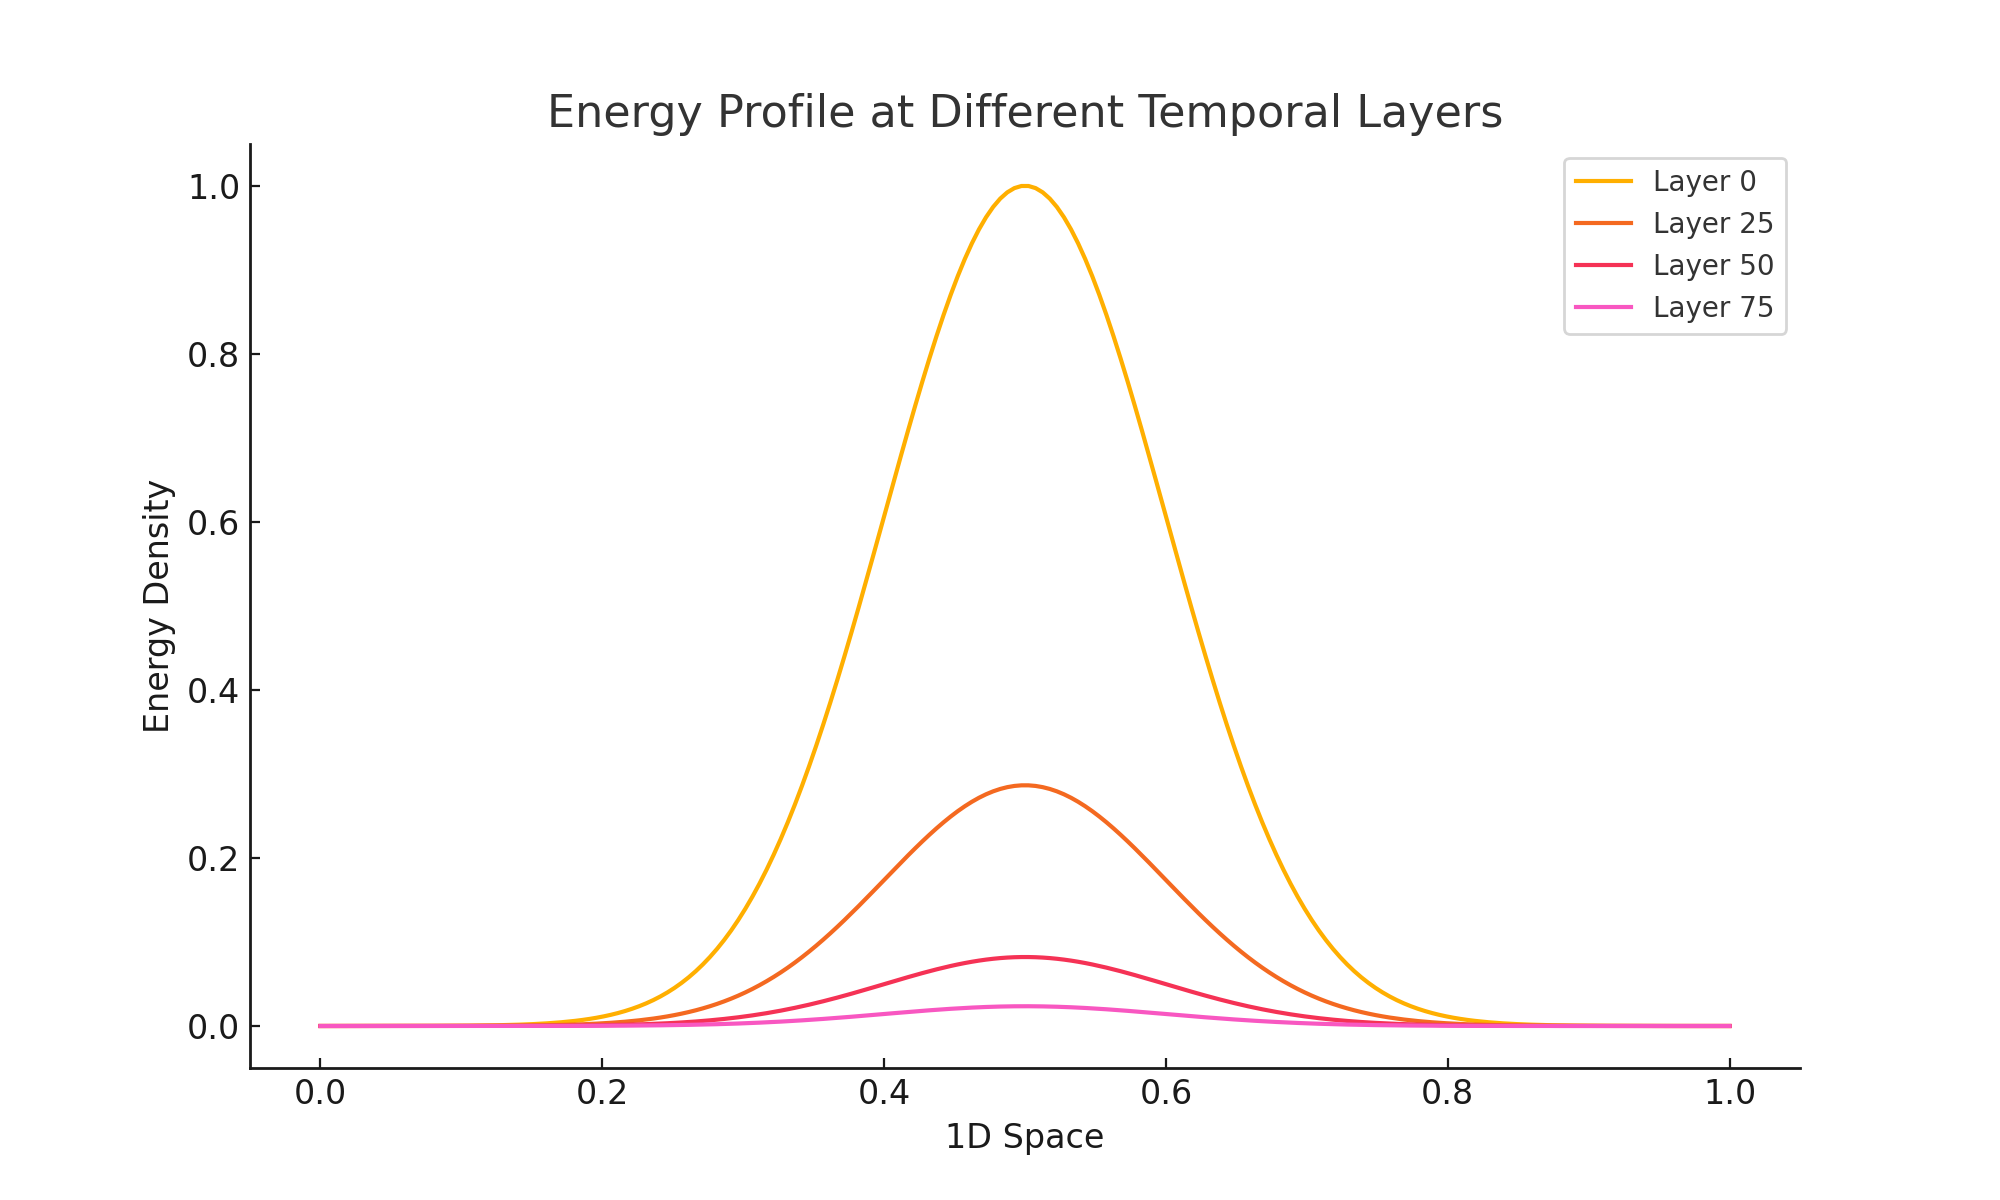
\includegraphics[width=0.9\linewidth]{05_Simulations/energy_profiles.png}
\caption{SVM Figure 1}
\label{fig:svm_1}
\caption{Energy profiles across temporal layers. Each curve represents the energy density distribution at a given discrete temporal layer.}
\end{figure}

\begin{figure}[h!]
\centering
\centering
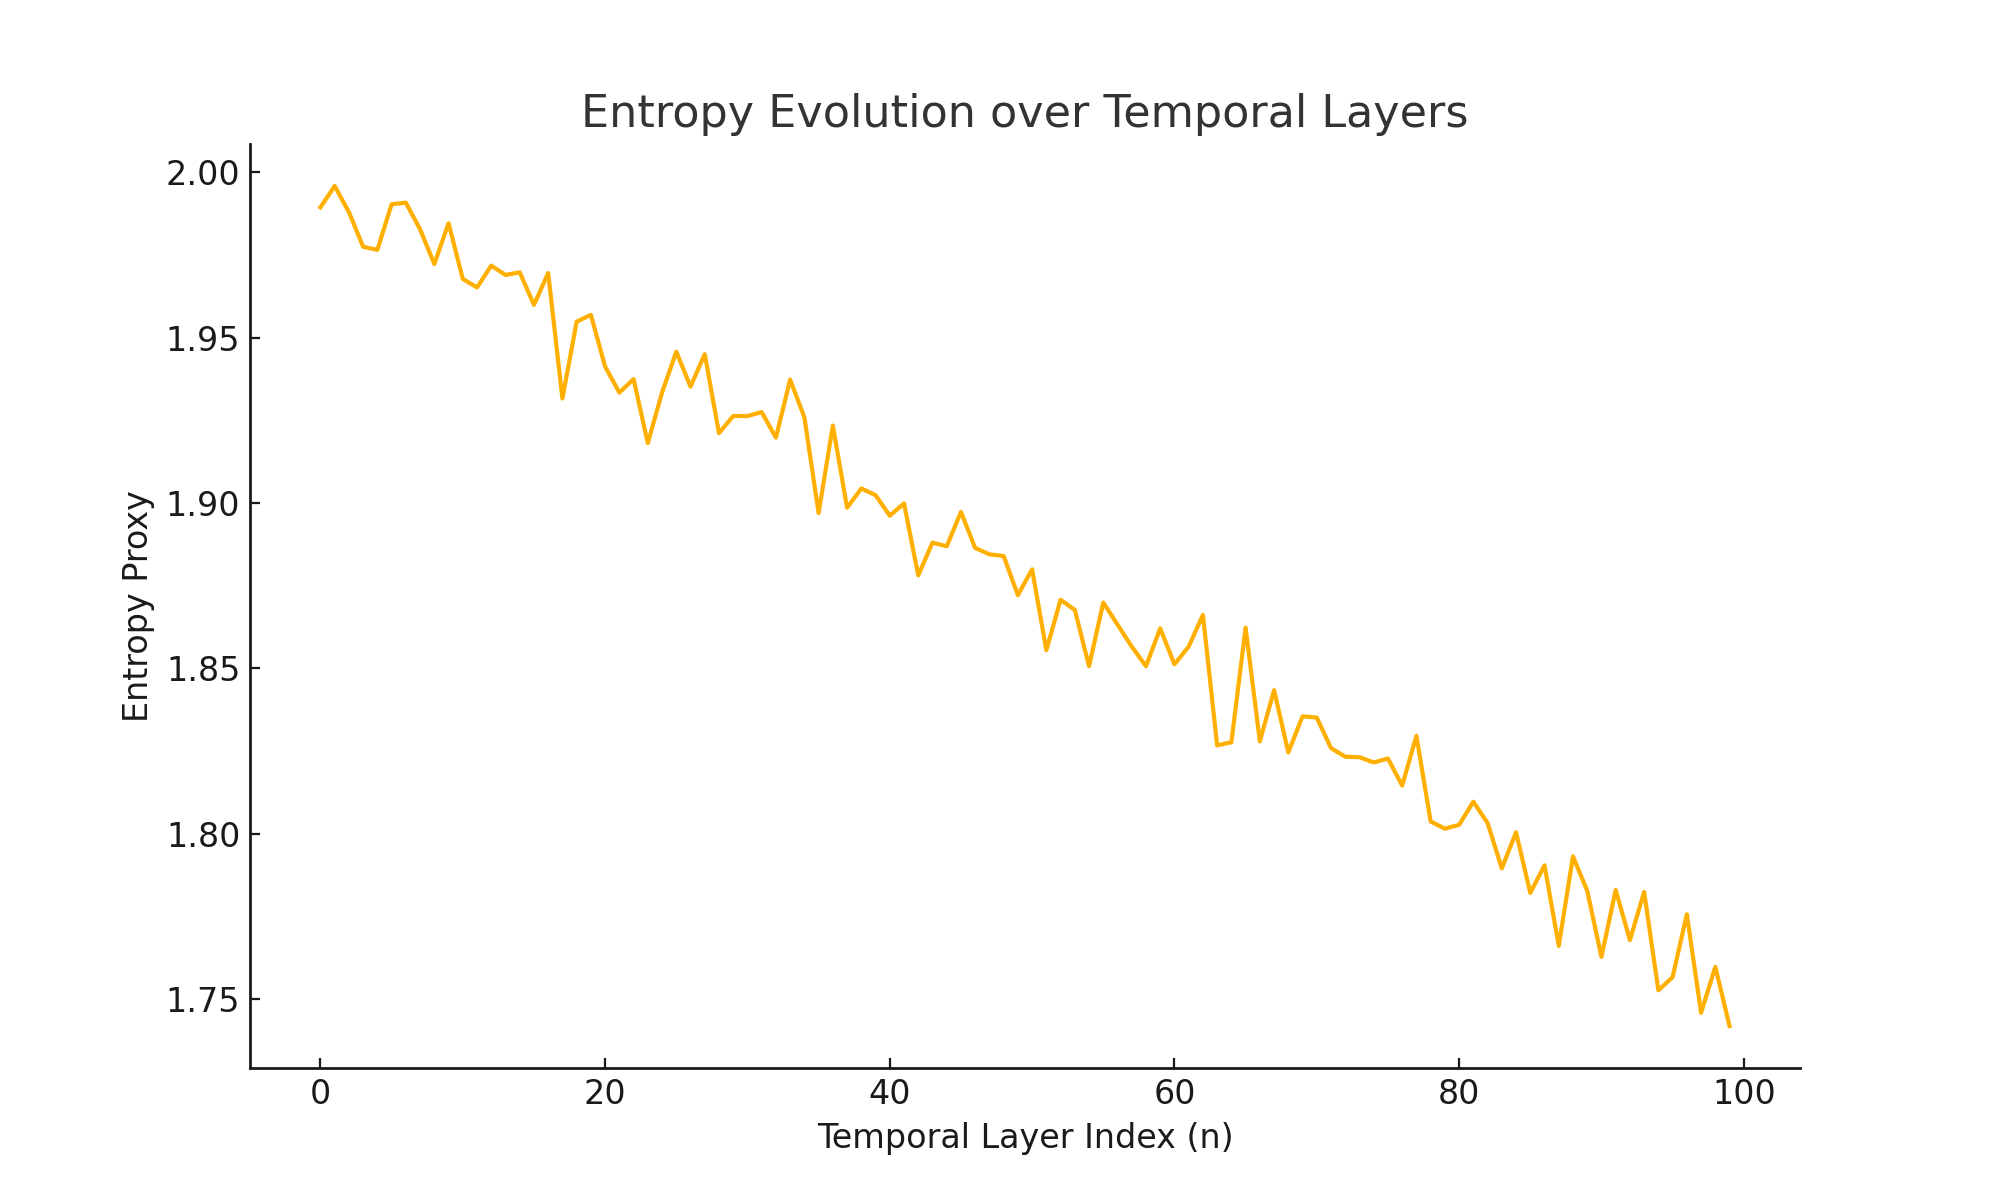
\includegraphics[width=0.9\linewidth]{05_Simulations/entropy_evolution.png}
\caption{SVM Figure 2}
\label{fig:svm_2}
\caption{Entropy evolution as a function of temporal layer index $n$. The slight decrease simulates entropic decay modulated by stochastic noise.}
\end{figure}

\begin{figure}[h!]
\centering
\centering
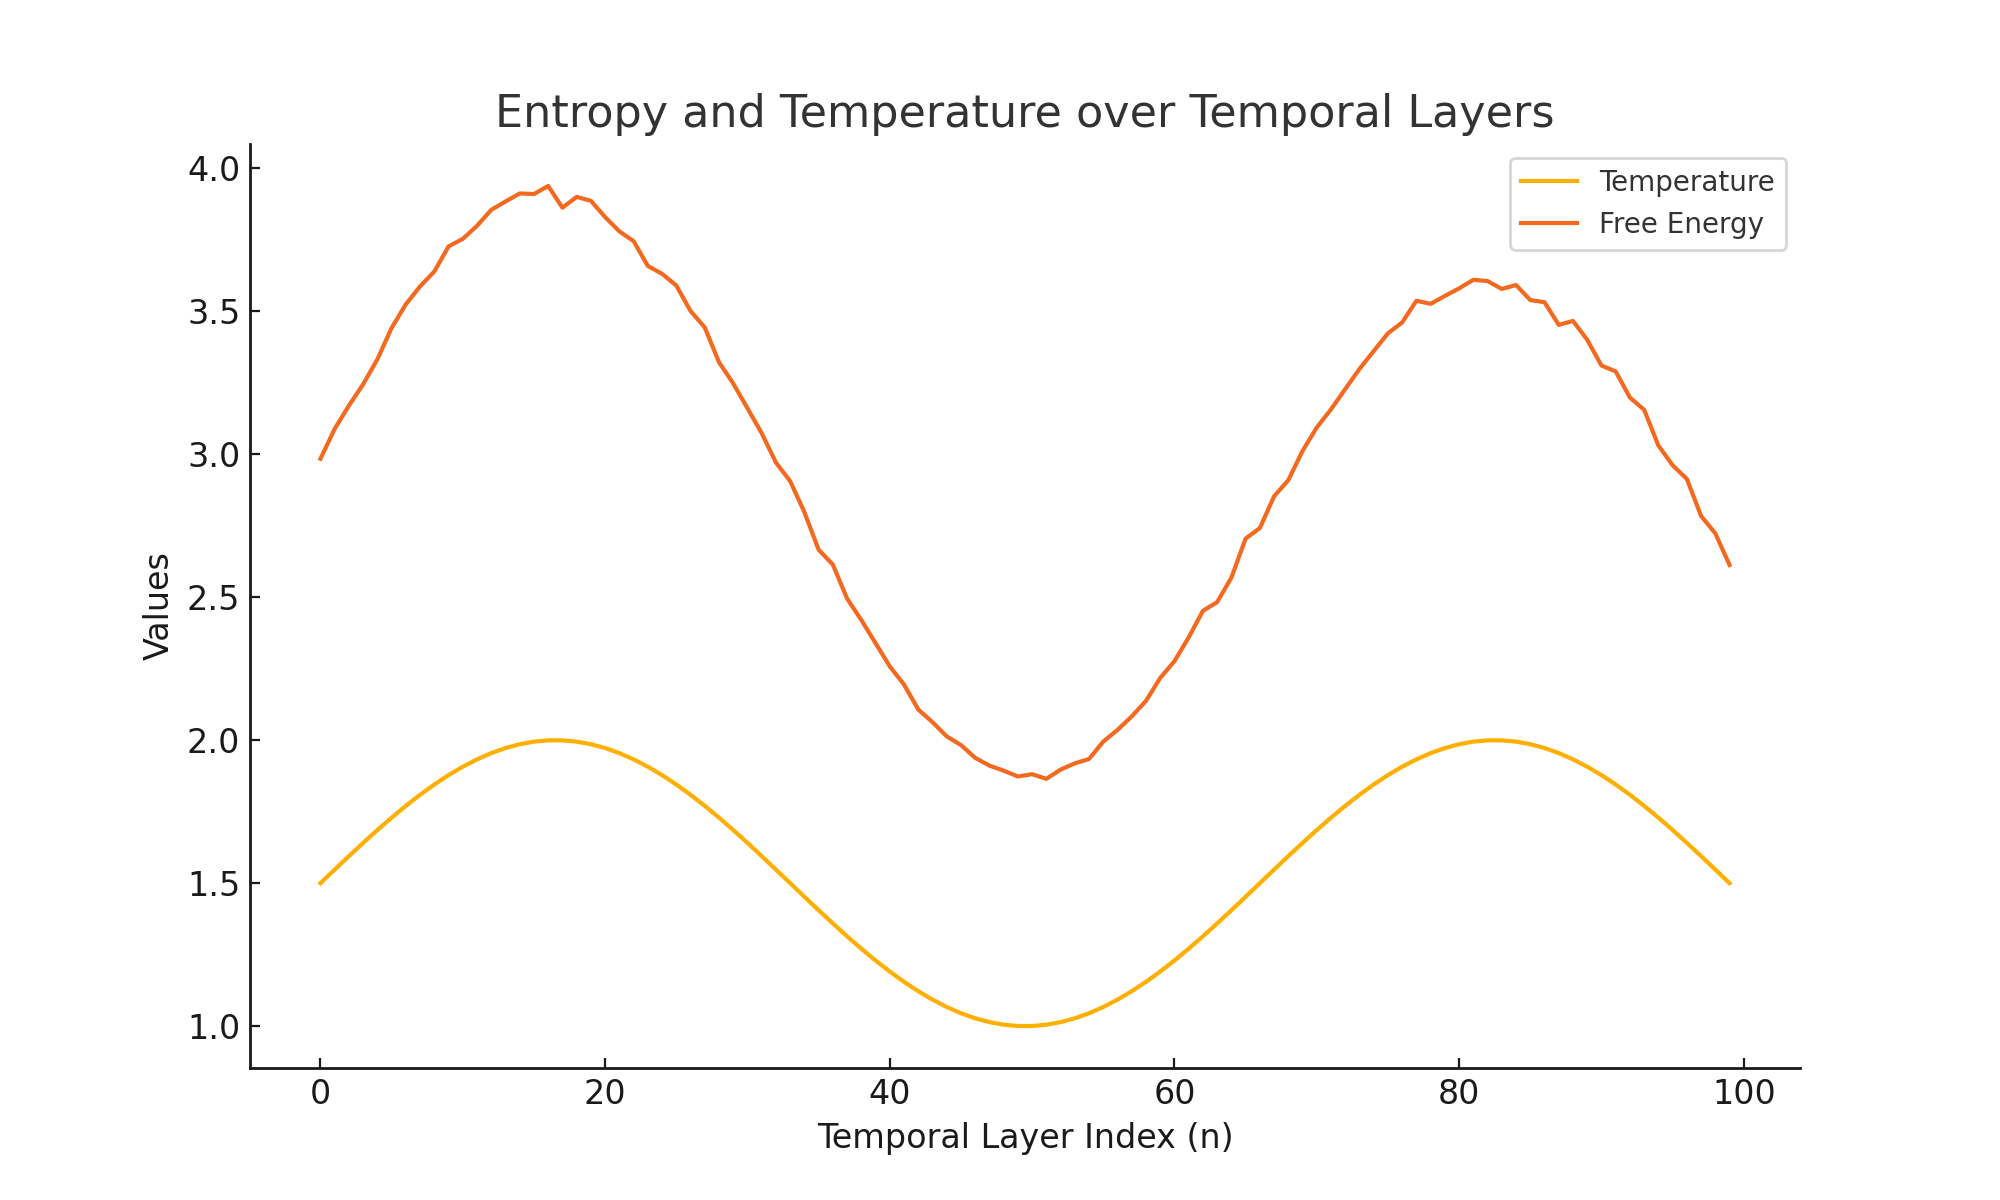
\includegraphics[width=0.9\linewidth]{05_Simulations/temp_free_energy.png}
\caption{SVM Figure 3}
\label{fig:svm_3}
\caption{Comparison of simulated temperature and free energy over time. Fluctuations are synthetic but reflect thermodynamic oscillations.}
\end{figure}

\begin{figure}[h!]
\centering
\centering
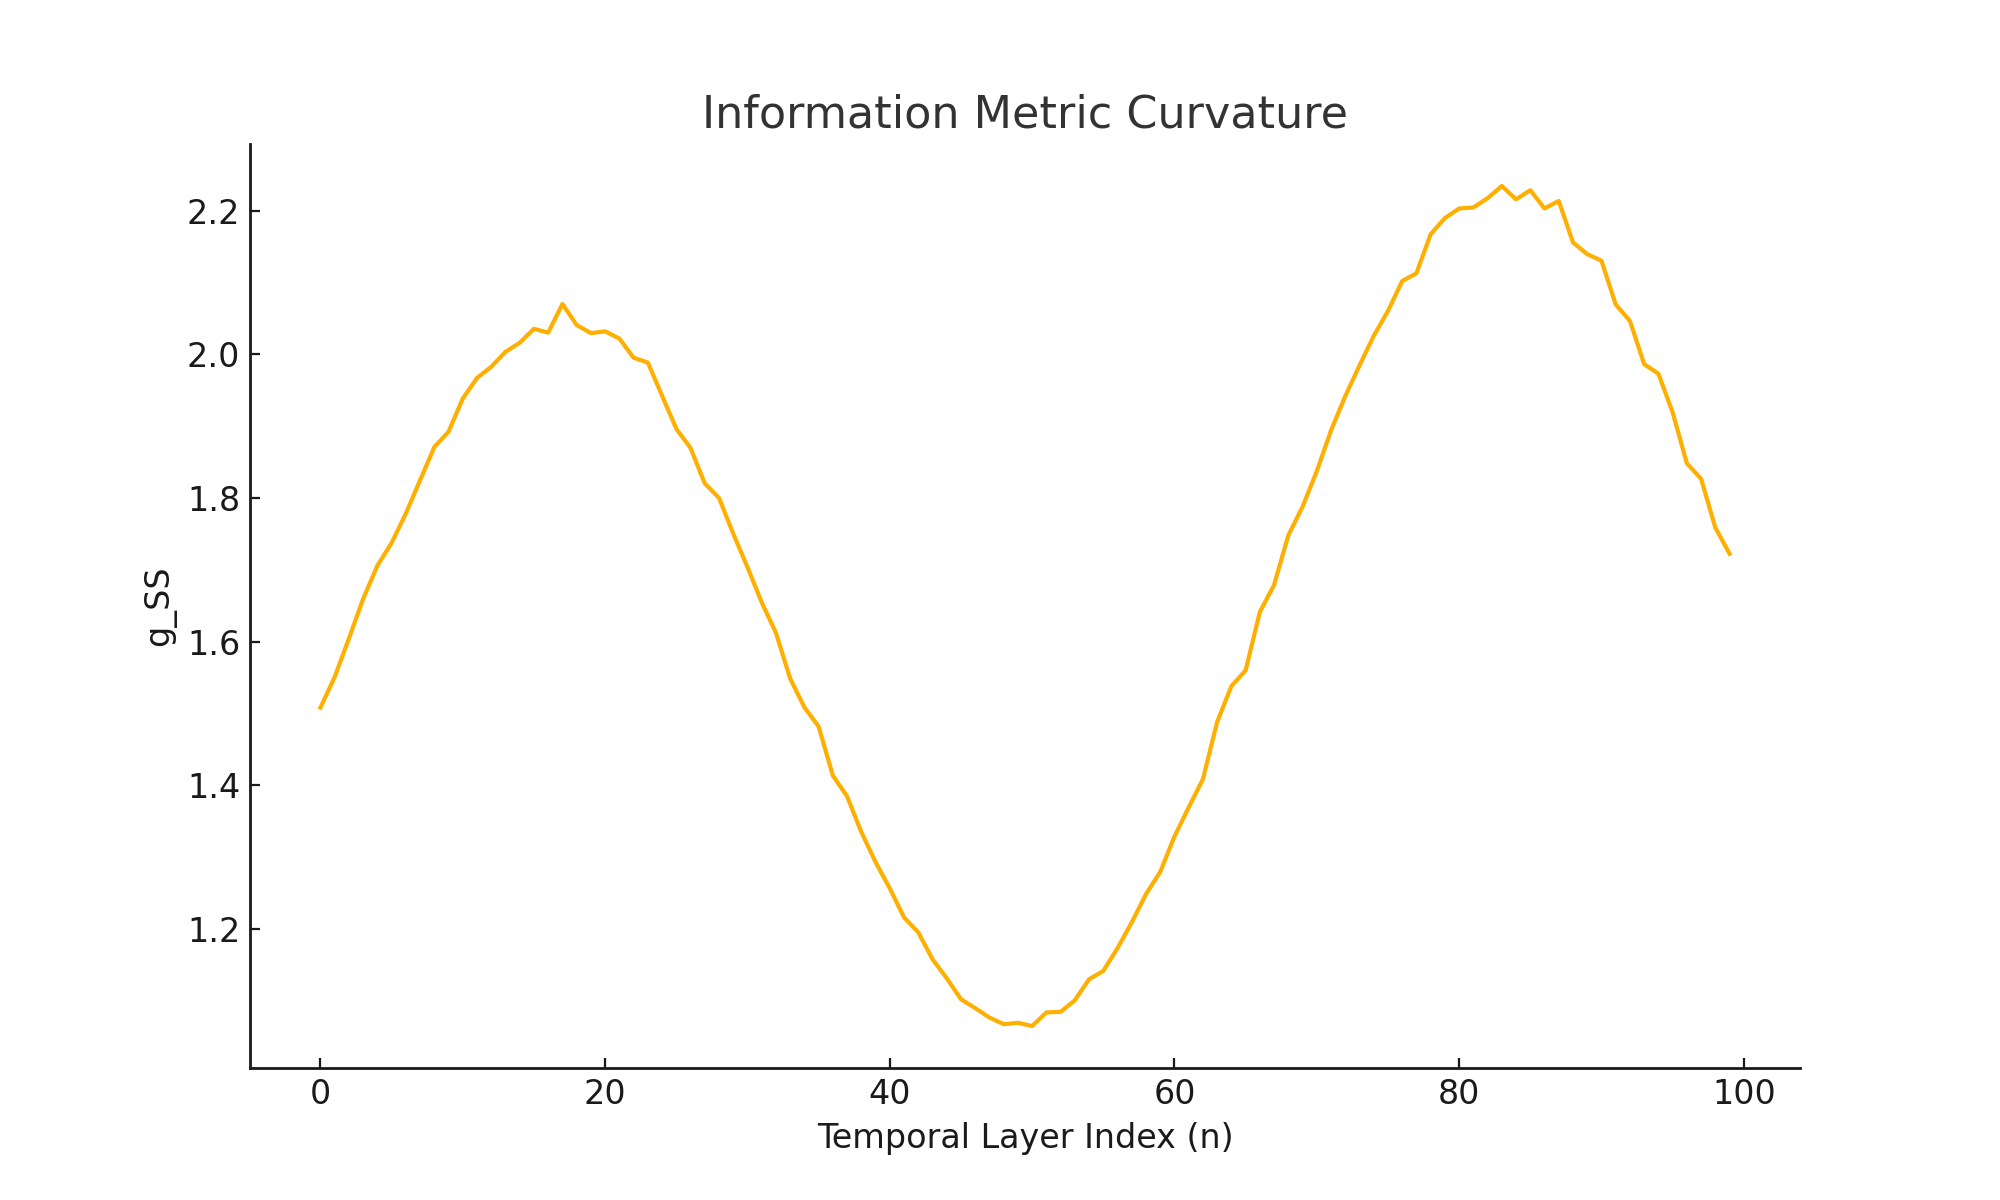
\includegraphics[width=0.9\linewidth]{05_Simulations/info_metric_curvature.png}
\caption{SVM Figure 4}
\label{fig:svm_4}
\caption{Information metric curvature $g_{SS}$ derived from synthetic entropy and temperature series.}
\end{figure}



\section{Model Comparison}

We compare the Spaciotemporal Vortex Model (SVM) with several major cyclic or quantum cosmological frameworks.

\begin{table}[htbp]
\centering
\footnotesize
\begin{tabularx}{\textwidth}{|l|X|X|X|X|X|X|}
\hline
\textbf{Model} & \textbf{Time Structure} & \textbf{Spacetime} & \textbf{Entropy Reset} & \textbf{Cyclicity} & \textbf{Thermodynamics} & \textbf{Quantum Gravity} \\
\hline
\textbf{SVM} & Layered, spatialized & Discrete 4D vortex & Yes, via collapse & Yes & Explicitly coupled & Formal extension via $\hat{S}_n$ \\
\textbf{CCC} & Conformal time loops & Classical, conformally rescaled & Yes, via conformal scaling & Yes & Not primary & Implicit (Penrose conjecture) \\
\textbf{LQC} & Bounce at Planck density & Quantized FLRW geometry & Yes, via bounce & Yes & Emergent from field quantization & Canonical loop quantization \\
\textbf{CDT} & Time-like slicing & Triangulated discrete spacetime & No explicit reset & No & Not considered & Emergent from path integral \\
\textbf{Ekpyrotic} & Cyclic brane collisions & Higher-dimensional & Partial (via brane tension) & Yes & Weakly integrated & String/M-theory inspired \\
\textbf{Steady-State} & Infinite, linear & Continuous expansion & No & No & Violates entropy increase & Classical only \\
\hline
\end{tabularx}
\caption{Comparison of key features across several cyclic and quantum cosmological models.}
\end{table}

\medskip

SVM dist

\appendix
\section{Appendix: Mathematical and Computational Details}

\subsection*{A.1 Discrete Action Derivation}

We start from the discrete action:
\begin{equation*}
A = \sum_n \left[ \frac{1}{2} (\partial_n S)^2 - V(S_n) \right]
\end{equation*}

Applying the discrete Euler-Lagrange principle:
\begin{equation*}
\frac{\partial L}{\partial S_n} - \Delta \left( \frac{\partial L}{\partial (\Delta S_n)} \right) = 0
\end{equation*}

Leads to:
\begin{equation*}
S_{n+1} - 2S_n + S_{n-1} = - \frac{\partial V}{\partial S_n}
\end{equation*}

\subsection*{A.2 Numerical Integration Scheme}

To simulate energy and entropy dispersion across layers:
\begin{itemize}
  \item Discretize spatial domain using $x_i = i \Delta x$
  \item Time evolution: $S_{n+1}(x_i) = S_n(x_i) + f(\Delta E_n(x_i))$
  \item Use centered finite differences for $\nabla^2$:
\begin{equation*}
\nabla^2 E_n(x_i) \approx \frac{E_n(x_{i+1}) - 2E_n(x_i) + E_n(x_{i-1})}{\Delta x^2}
\end{equation*}
\end{itemize}

\subsection*{A.3 Thermodynamic Relations}

Recall:
\begin{align*}
Q_n &= c_v T_n \\
F(S_n) &= S_n T_n \\
g_{ab} &= \partial_a \partial_b F(S_n) \\
\Delta S_n &= \frac{\Delta Q_n}{T_n} + \sigma_n \geq 0
\end{align*}

This structure forms a thermal-geometric space where entropy, temperature, and curvature are coevolving.

\section{Discrete Spatial Layers}
We define a 4-dimensional space \( S^4 \) that includes the three spatial dimensions \( x, y, z \) and a fourth spatial dimension \( t_s \) representing discrete "time-layers".

Formally, the 
at a given layer \( n \) can be described by:

\begin{equation}
U_n = \{ (x, y, z, t_s) \mid t_s = n, n \in \mathbb{Z} \}
\end{equation}

Each layer \(U_n\) contains a complete spatial distribution of energy \(E_n(x, y, z)\).

\section{Energy Transition Between Layers}

The transition between layers \( U_n \) to \( U_{n+1} \) is governed by the transfer of energy. We postulate an energy transition operator \(T\), defined as:

\begin{equation}
T: U_n \rightarrow U_{n+1}, \quad T(E_n) = E_{n+1}
\end{equation}

Energy conservation across layers is given by:

\begin{equation}
\int_{-\infty}^{+\infty}\int_{-\infty}^{+\infty}\int
\end{equation}

\section{Cyclic Collapse and Reinitialization of Interactive Spacetime}

At the critical timestep \( n_{\mathrm{crit}} = 2\tau \cdot 10^{40} \), the expansion of the universe reaches a scale 
at that all known fundamental interactions become ineffective. The average distance between particles 

\( r(n) \sim \sqrt{n / (2\tau)} \) exceeds the maximum effective range \( d_{\mathrm{interact}} \sim 10^{20} \ell_P \).


This initiates a phase of entropic stagnation: energy becomes non-interactive and falls backward 
through the fourth spatial dimension. Compression through shrinking temporal hypersurfaces eventually reconverges 
all energy at the singularity-like point \([X,Y,Z,T] = [0,0,0,0]\).


Interaction is reactivated when the radius satisfies:

\begin{equation*}
I(n) = \frac{1}{1 + \exp\left(-\alpha (d_{\mathrm{interact}} - \sqrt{n / (2\tau)})\right)}
\end{equation*}

with \( \alpha \sim 10^{18} \), describing a Planck-scale transition.

The interactive energy field re-activates and explosively expands, constituting the next Big Bang. 

We model this using a tensor field:

\begin{equation*}
\mathcal{I}_{\mu\nu}(x,n) = I(n) \cdot \rho(x,n) \cdot g_{\mu\nu}
\end{equation*}

and modified field equations:

\begin{equation*}
G_{\mu\nu} = \kappa \, \mathcal{I}_{\mu\nu}
\end{equation*}

See Figures~\ref{fig:spacetimecone}, \ref{fig:energydensity}, \ref{fig:interactivitystate}.

\section{Physical Parameterization in SI Units}

The spaciotemporal vortex model is grounded in Planck-scale discretization, allowing translation into SI units:

\begin{itemize}
  \item Planck Time: $t_P = 5.39 \times 10^{-44} \, \mathrm{s}$
  \item Planck Length: $\ell_P = 1.62 \times 10^{-35} \, \mathrm{m}$
  \item Planck Energy: $E_P = 1.96 \times 10^{9} \, \mathrm{J}$
  \item Planck Energy Density: $\rho_P = 4.63 \times 10^{113} \, \mathrm{J/m^3}$
\end{itemize}

At the critical timestep $n_{\mathrm{crit}} \approx 2 \cdot 10^{40}$, the model yields:

\begin{itemize}
  \item Radius: $r(n_{\mathrm{crit}}) \approx 1.62 \times 10^{-15} \, \mathrm{m}$
  \item Elapsed time: $t(n_{\mathrm{crit}}) \approx 1.08 \times 10^{-3} \, \mathrm{s}$
\end{itemize}

As $r(n) \rightarrow \ell_P$, energy density converges toward:

\begin{equation*}
\rho(n) \rightarrow \frac{E_P}{\ell_P^3} \approx 4.63 \times 10^{113} \, \mathrm{J/m^3}
\end{equation*}

\begin{figure}[ht]
\centering
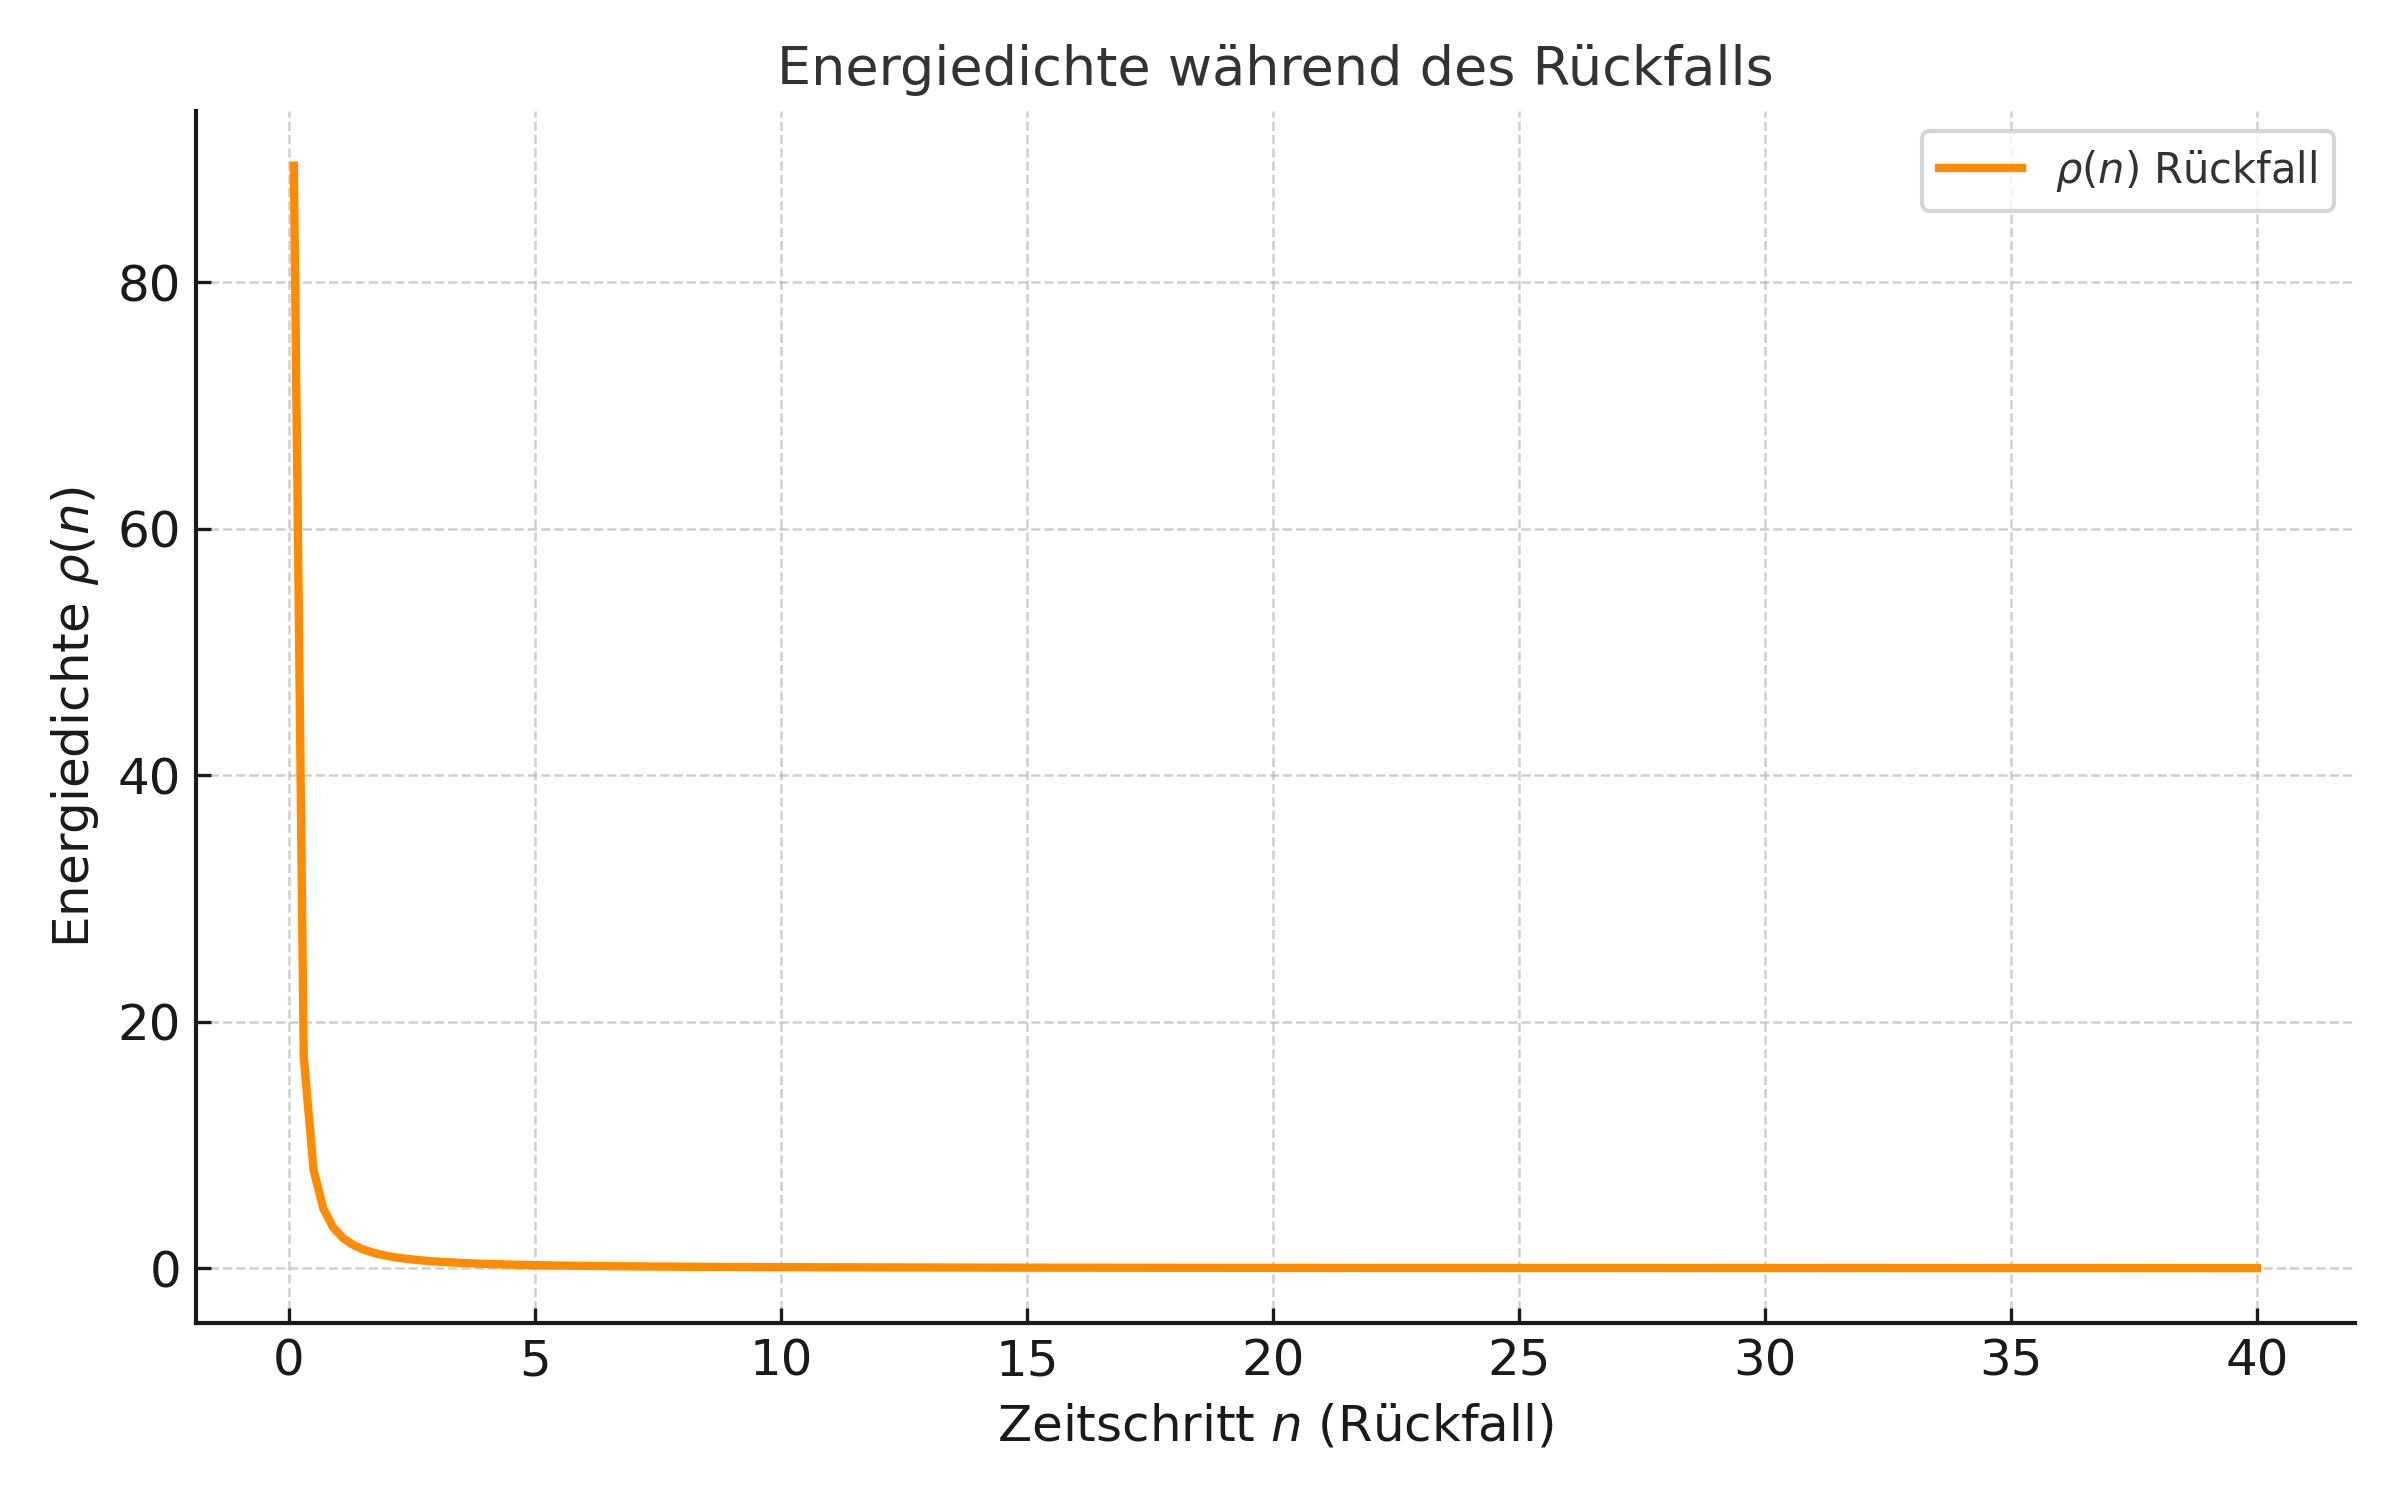
\includegraphics[width=0.85\textwidth]{figures/SVM_Energy_Density_Recollapse.png}
\caption{SVM Figure 5}
\label{fig:svm_5}
\caption{Energy density increase during the recollapse phase approaching Planck-scale compression.}\label{fig:energydensity}
\end{figure}

\begin{figure}[ht]
\centering
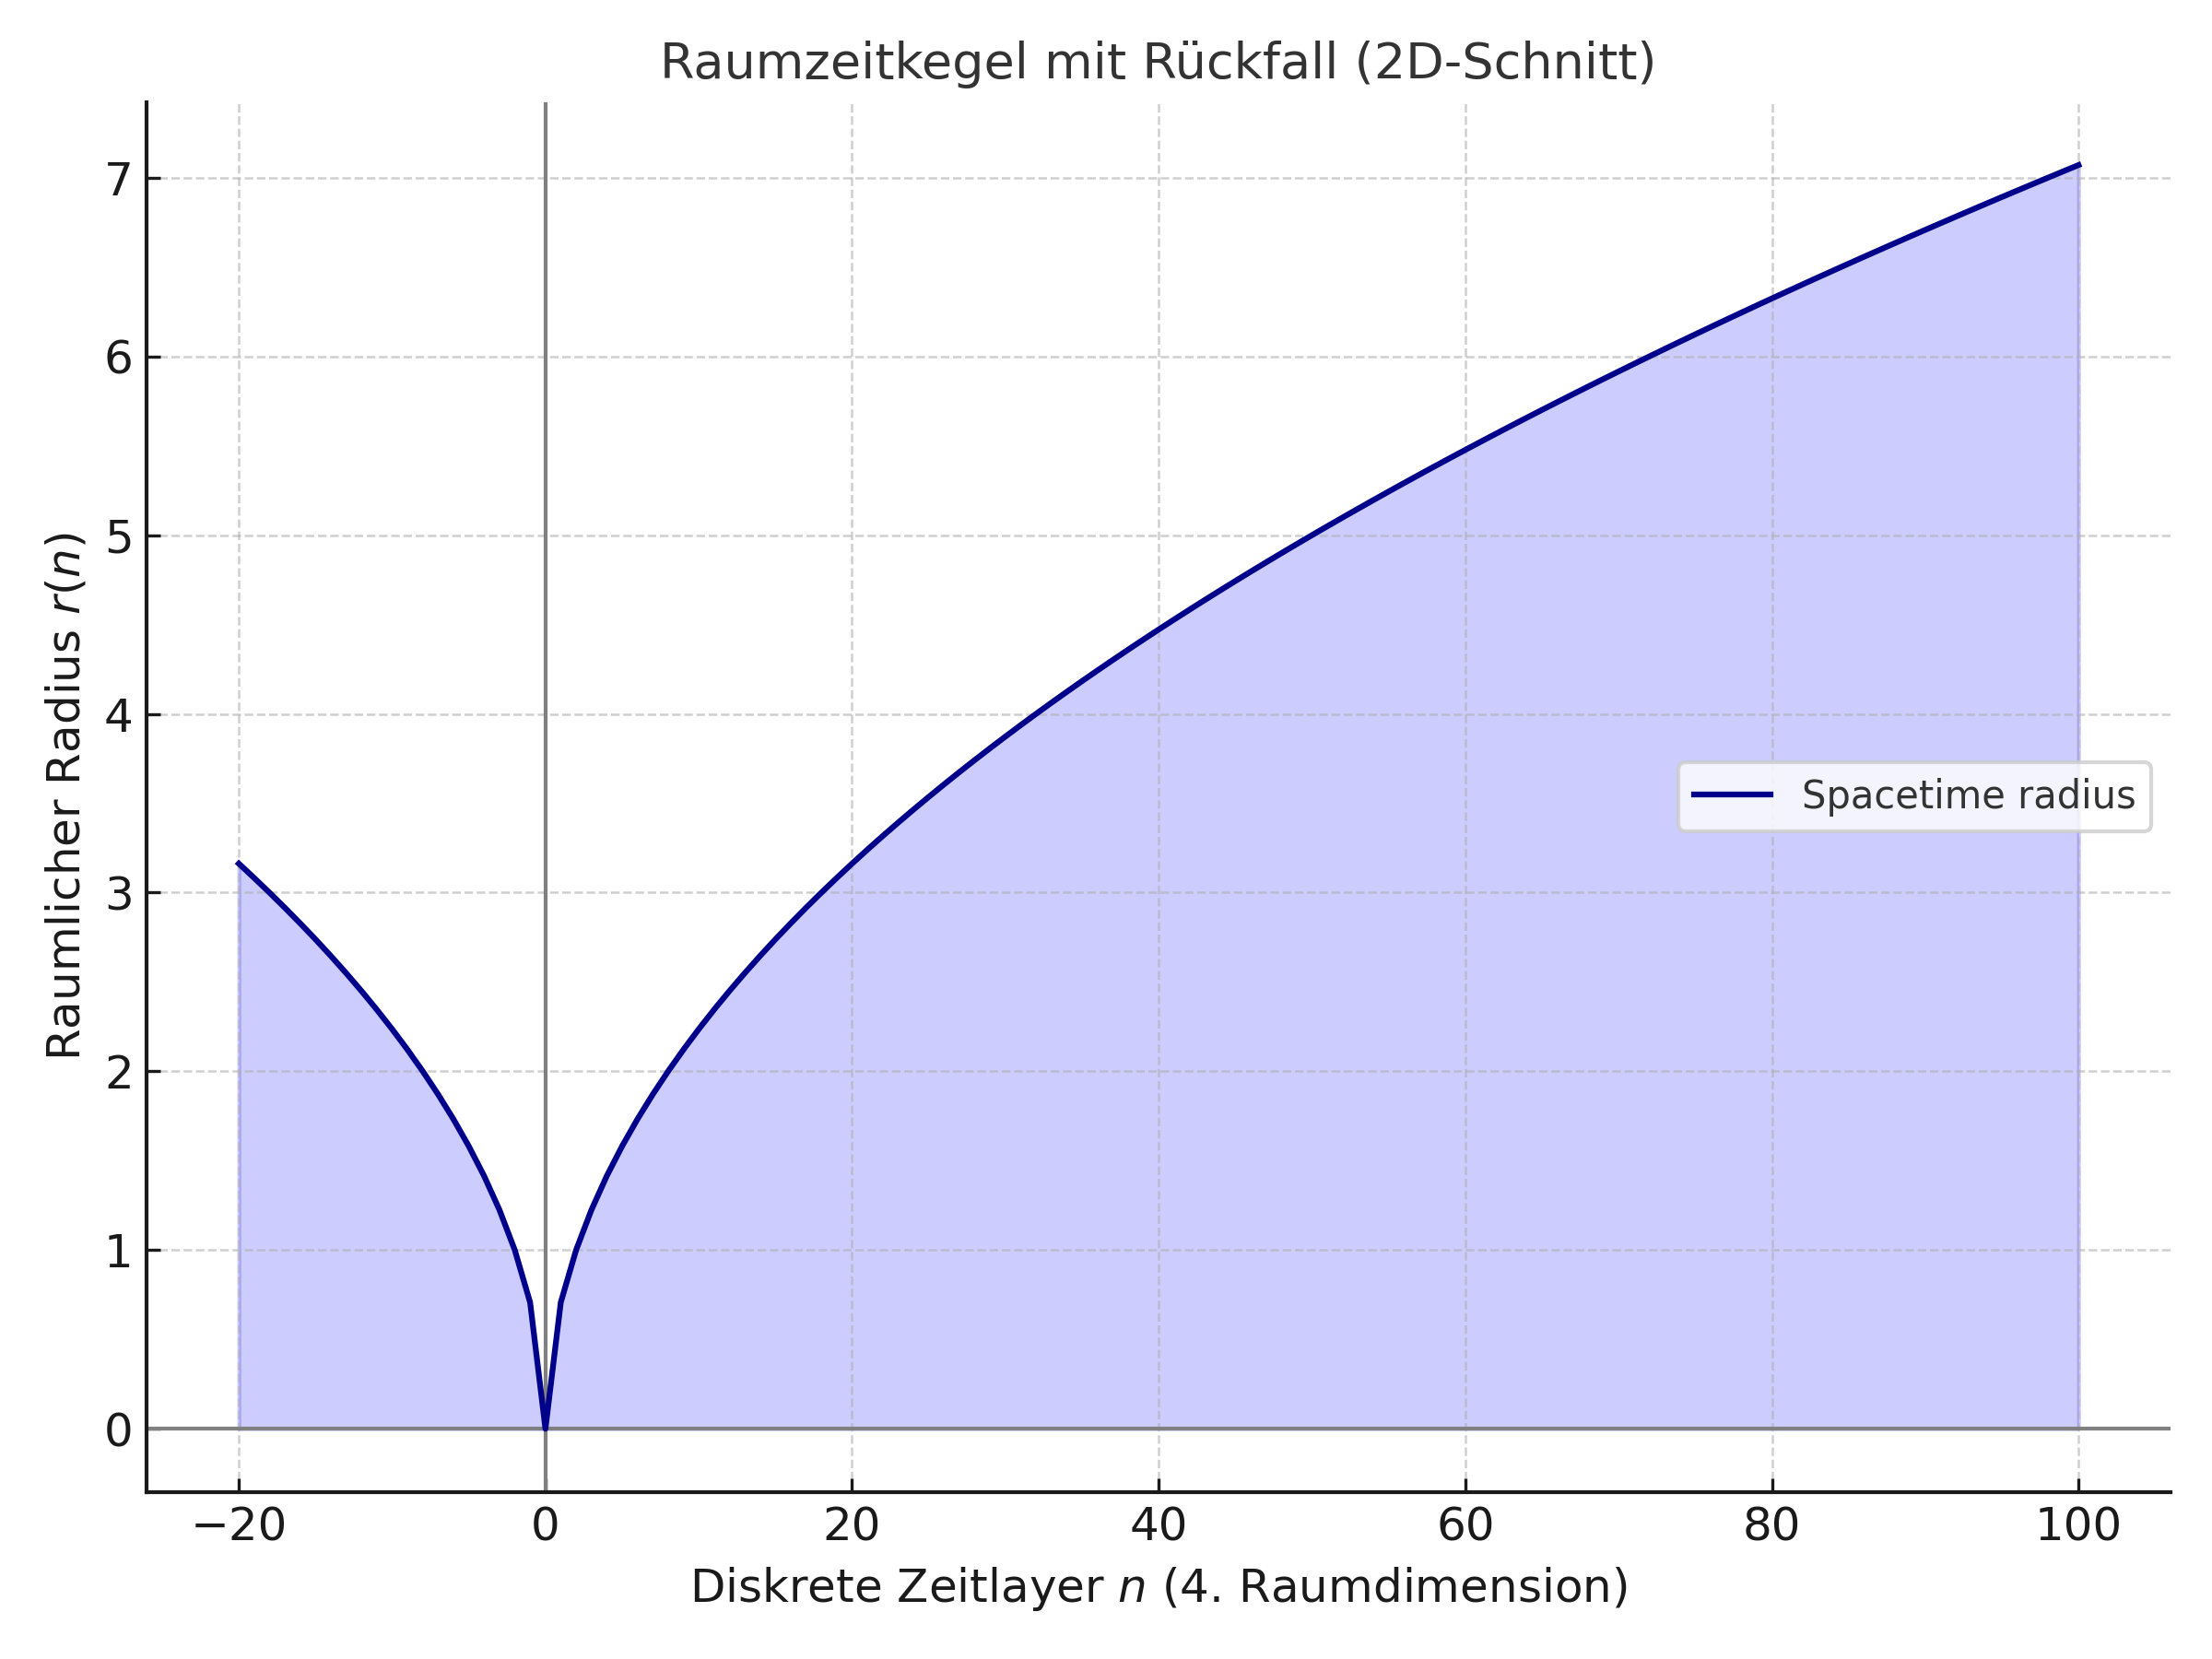
\includegraphics[width=0.85\textwidth]{figures/SVM_Spacetime_Cone_With_Recollapse.png}
\caption{SVM Figure 6}
\label{fig:svm_6}
\caption{Spacetime cone visualization showing forward expansion and backward collapse through Planck time layers.}\label{fig:spacetimecone}
\end{figure}

\section{References}
\
\bibliographystyle{plain}
\begin{enumerate}
    \item \cite{ambjorn2012nonperturbative}
    \item \cite{ashtekar2006quantum}
    \item \cite{baum2020thermal}
    \item \cite{penrose2010cycles}
\end{enumerate}
\bibliography{svm_bibliography.bib}


\section*{Abstract}

The Spaciotemporal Vortex Model (SVM) offers a physically grounded framework in which time is reinterpreted as a layered fourth spatial dimension. Temporal evolution results from energy transitions between discrete temporal layers. Unlike conventional cosmological models, which treat time as a continuous linear axis and fail to address the low-entropy initial state, arrow of time, or dark phenomena, SVM introduces a novel mechanism: gravitational resistance to inter-layer transitions. This reinterpretation provides a thermodynamically coherent basis for cyclic cosmological dynamics, entropy management, and information encoding via curvature. The model derives formal evolution laws, thermodynamic couplings, and quantization paths, offering multiple empirical implications for entropy collapse, dark energy behavior, and curvature-entropy correspondence.


\section{Introduction}

Contemporary cosmological models based on General Relativity conceptualize time as a linear, continuous dimension, fundamentally distinct from space. However, they leave unresolved several foundational problems:

\begin{itemize}
    \item The origin of the arrow of time,
    \item The mechanism behind the universe's extremely low initial entropy,
    \item The nature of dark matter and dark energy,
    \item The inability to naturally implement cyclic or entropy-resetting cosmologies.
\end{itemize}

The Spaciotemporal Vortex Model (SVM) introduces a restructured interpretation of time as a layered, discretized spatial dimension. Energy transitions between these temporal layers define temporal progression. Gravitational interactions are reinterpreted as impedance to such transitions. This framework offers a thermodynamically coupled, cyclic cosmology that is ontologically novel, mathematically formalized, and empirically tractable.


\subsection*{Operator Definition}

Let $f(\Delta E_n(x)) := \alpha \, \nabla^2 \Delta E_n(x)$ with $\alpha$ a dimensionless scaling factor.

The temporal layer transition becomes:
\begin{equation*}
S_{n+1}(x) = S_n(x) + \alpha \nabla^2 \Delta E_n(x)
\end{equation*}

Where $\nabla^2$ introduces spatial locality and diffusion-like behavior. If $[\Delta E] = \mathrm{J/m^3}$, then:

\begin{equation*}
[f(\Delta E)] = \mathrm{J/m^5}
\quad \Rightarrow \quad [S_{n+1}] = [S_n] + \mathrm{J/m^5}
\end{equation*}

\subsection*{Symbol Analysis}

\begin{tabular}{|c|l|l|c|}
\hline
Symbol & Meaning & Unit/Type & Consistent? \\
\hline
$S_n$ & State per temporal layer & Energy distribution & Yes \\
$\pi_n$ & Transition momentum & Energy per layer & Yes \\
$T_n$ & Temperature in layer & [K] & Yes \\
$Q_n$ & Heat transfer & [J] & Yes \\
\hline
\end{tabular}


\section{Quantum Thermodynamic Extension}

To extend the spaciotemporal model toward a quantum thermodynamic formalism, we promote the classical variables to operators:

\begin{equation*}
\hat{S}_n, \quad \hat{\pi}_n, \quad [\hat{S}_n, \hat{\pi}_n] = i\hbar
\end{equation*}

The discrete action becomes a quantum path sum over all possible layer evolutions:

\begin{equation*}
Z = \sum_{\text{paths}} e^{-A[S]/\hbar}
\end{equation*}

Including quantum fluctuations of entropy and temperature:

\begin{equation*}
Z = \int \mathcal{D}S\, \mathcal{D}T\, \mathcal{D}Q\, e^{- \sum_n L(S_n, T_n, Q_n)/\hbar}
\end{equation*}

This formulation allows for a quantum statistical interpretation of interlayer dynamics, where temporal evolution reflects probabilistic thermal behavior.



\section{Information Geometry}

We define a Riemannian metric over the thermodynamic layer state space $\Omega_n := \{S_n, \pi_n, T_n, Q_n\}$ using curvature of the free energy $F(S_n)$:

\begin{equation*}
g_{ab} = \partial_a \partial_b F(S_n)
\end{equation*}

In terms of statistical physics, this corresponds to:

\begin{equation*}
g_{ab} = -\partial_a \partial_b \log Z
\end{equation*}

The metric captures fluctuations and geodesic paths in the thermodynamic manifold. The curvature $R$ of this manifold may be interpreted as encoding gravitational analogues in the SVM framework.





\section{Model Comparison}

We compare the Spaciotemporal Vortex Model (SVM) with several major cyclic or quantum cosmological frameworks.

\begin{table}[htbp]
\centering
\footnotesize
\begin{tabularx}{\textwidth}{|l|X|X|X|X|X|X|}
\hline
\textbf{Model} & \textbf{Time Structure} & \textbf{Spacetime} & \textbf{Entropy Reset} & \textbf{Cyclic~\cite{steinhardt2002cyclic}ity} & \textbf{Thermodynamics} & \textbf{Quantum Gravity} \\
\hline
\textbf{SVM} & Layered, spatialized & Discrete 4D vortex & Yes, via collapse & Yes & Explicitly coupled & Formal extension via $\hat{S}_n$ \\
\textbf{CCC} & Conformal time loops & Classical, conformally rescaled & Yes, via conformal scaling & Yes & Not primary & Implicit (Penrose~\cite{penrose2010cycles} conjecture) \\
\textbf{LQC} & Bounce at Planck density & Quantized FLRW geometry & Yes, via bounce & Yes & Emergent from field quantization & Canonical loop quantization \\
\textbf{CDT} & Time-like slicing & Triangulated discrete spacetime & No explicit reset & No & Not considered & Emergent from path integral \\
\textbf{Ekpyrotic} & Cyclic brane collisions & Higher-dimensional & Partial (via brane tension) & Yes & Weakly integrated & String/M-theory inspired \\
\textbf{Steady-State} & Infinite, linear & Continuous expansion & No & No & Violates entropy increase & Classical only \\
\hline
\end{tabularx}
\caption{Comparison of key features across several cyclic and quantum cosmological models.}
\end{table}

\medskip

SVM distinguishes itself by integrating time as a spatial layer dimension and offering a fully thermodynamic-coupled formalism including entropy, temperature, and free energy evolution. It supports empirical modeling via geometric curvature and quantum entropy fluctuations.


\section{Conclusion and Outlook}

The Spaciotemporal Vortex Model (SVM) provides a physically motivated and mathematically consistent alternative to conventional cosmological models by redefining time as a layered spatial dimension. This ontological shift allows energy and entropy to evolve along discrete temporal transitions, which are interpreted as physical processes rather than abstract parameters.

\subsection*{Empirical Priorities}

Key avenues for future empirical investigation include:
\begin{itemize}
    \item Detection of entropy-curvature correlations in the CMB.
    \item Searching for discrete imprints or "layer scars" in gravitational wave spectra.
    \item Investigating temperature fluctuations tied to quantum entropy effects.
\end{itemize}

\subsection*{Computational Tasks}

We aim to simulate:
\begin{itemize}
    \item Layered state evolutions using finite-difference or finite-element methods.
    \item Entropy dispersion as geometric diffusion in $\Omega_n$.
    \item Free energy landscapes and curvature-induced state changes.
\end{itemize}

\subsection*{Theoretical Development}

Future refinements of the model will involve:
\begin{itemize}
    \item Tensorial formulations of $g_{ab}$ with curvature invariants.
    \item Deriving gravitational field equations based on thermodynamic conjugates.
    \item Incorporating black hole boundary layers as entropy flux gates.
\end{itemize}

SVM proposes a coherent language that bridges thermodynamic irreversibility, quantum uncertainty, and geometric structure. Continued development will focus on rendering this framework testable, implementable, and compatible with fundamental physical constraints.


\appendix
\section{Appendix: Mathematical and Computational Details}

\subsection*{A.1 Discrete Action Derivation}

We start from the discrete action:
\begin{equation*}
A = \sum_n \left[ \frac{1}{2} (\partial_n S)^2 - V(S_n) \right]
\end{equation*}

Applying the discrete Euler-Lagrange principle:
\begin{equation*}
\frac{\partial L}{\partial S_n} - \Delta \left( \frac{\partial L}{\partial (\Delta S_n)} \right) = 0
\end{equation*}

Leads to:
\begin{equation*}
S_{n+1} - 2S_n + S_{n-1} = - \frac{\partial V}{\partial S_n}
\end{equation*}

\subsection*{A.2 Numerical Integration Scheme}

To simulate energy and entropy dispersion across layers:
\begin{itemize}
  \item Discretize spatial domain using $x_i = i \Delta x$
  \item Time evolution: $S_{n+1}(x_i) = S_n(x_i) + f(\Delta E_n(x_i))$
  \item Use centered finite differences for $\nabla^2$:
\begin{equation*}
\nabla^2 E_n(x_i) \approx \frac{E_n(x_{i+1}) - 2E_n(x_i) + E_n(x_{i-1})}{\Delta x^2}
\end{equation*}
\end{itemize}

\subsection*{A.3 Thermodynamic Relations}

Recall:
\begin{align*}
Q_n &= c_v T_n \\
F(S_n) &= S_n T_n \\
g_{ab} &= \partial_a \partial_b F(S_n) \\
\Delta S_n &= \frac{\Delta Q_n}{T_n} + \sigma_n \geq 0
\end{align*}

This structure forms a thermal-geometric space where entropy, temperature, and curvature are co-evolving.



\section{Visualization of Layer Dynamics}

\begin{figure}[h!]
\centering
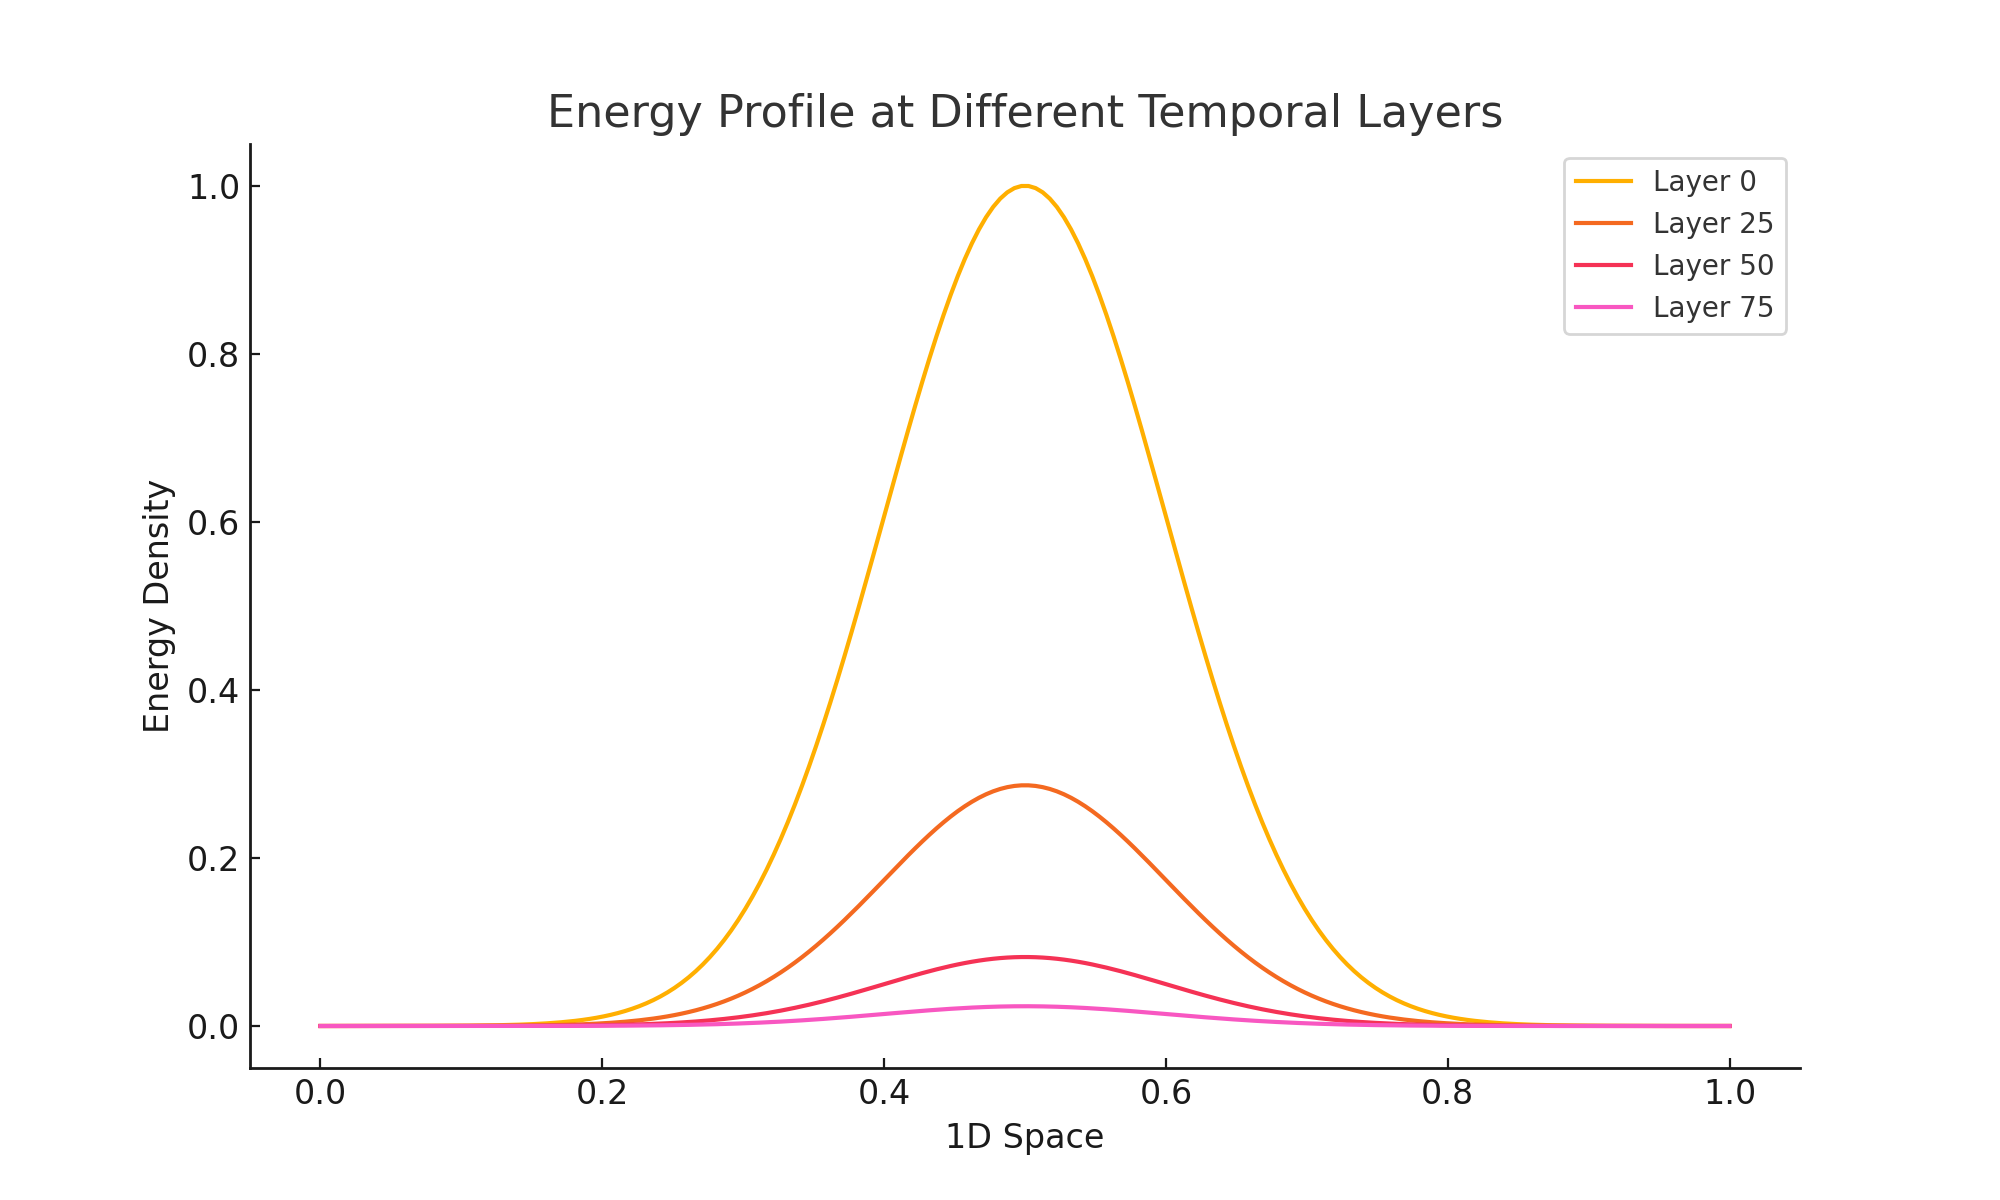
\includegraphics[width=0.9\linewidth]{05_Simulations/energy_profiles.png}
\caption{Energy profiles across temporal layers. Each curve represents the energy density distribution at a given discrete temporal layer.}\label{fig:interactivitystate}
\end{figure}

\begin{figure}[h!]
\centering
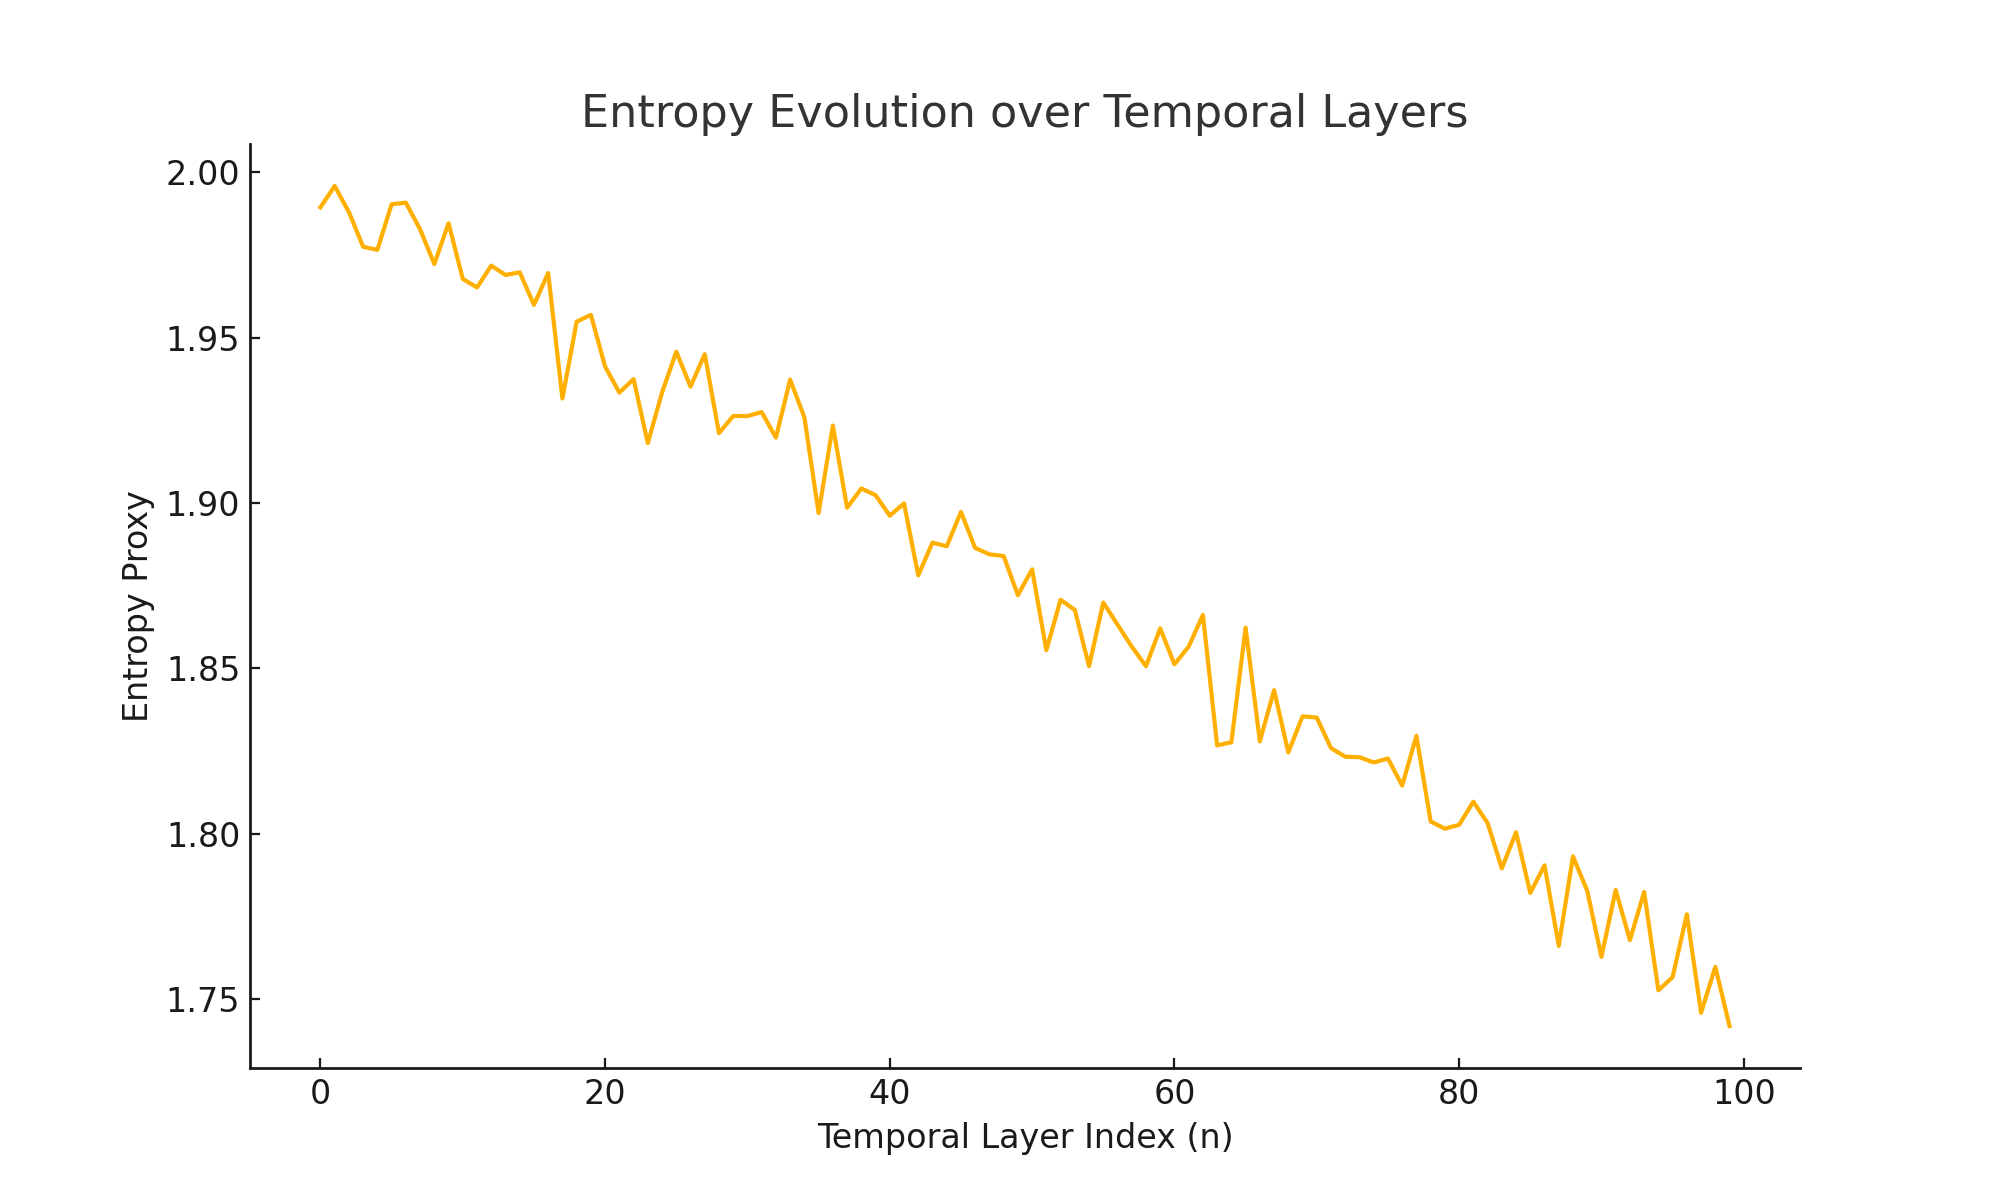
\includegraphics[width=0.9\linewidth]{05_Simulations/entropy_evolution.png}
\caption{Entropy evolution as a function of temporal layer index $n$. The slight decrease simulates entropic decay modulated by stochastic noise.}
\end{figure}

\begin{figure}[h!]
\centering
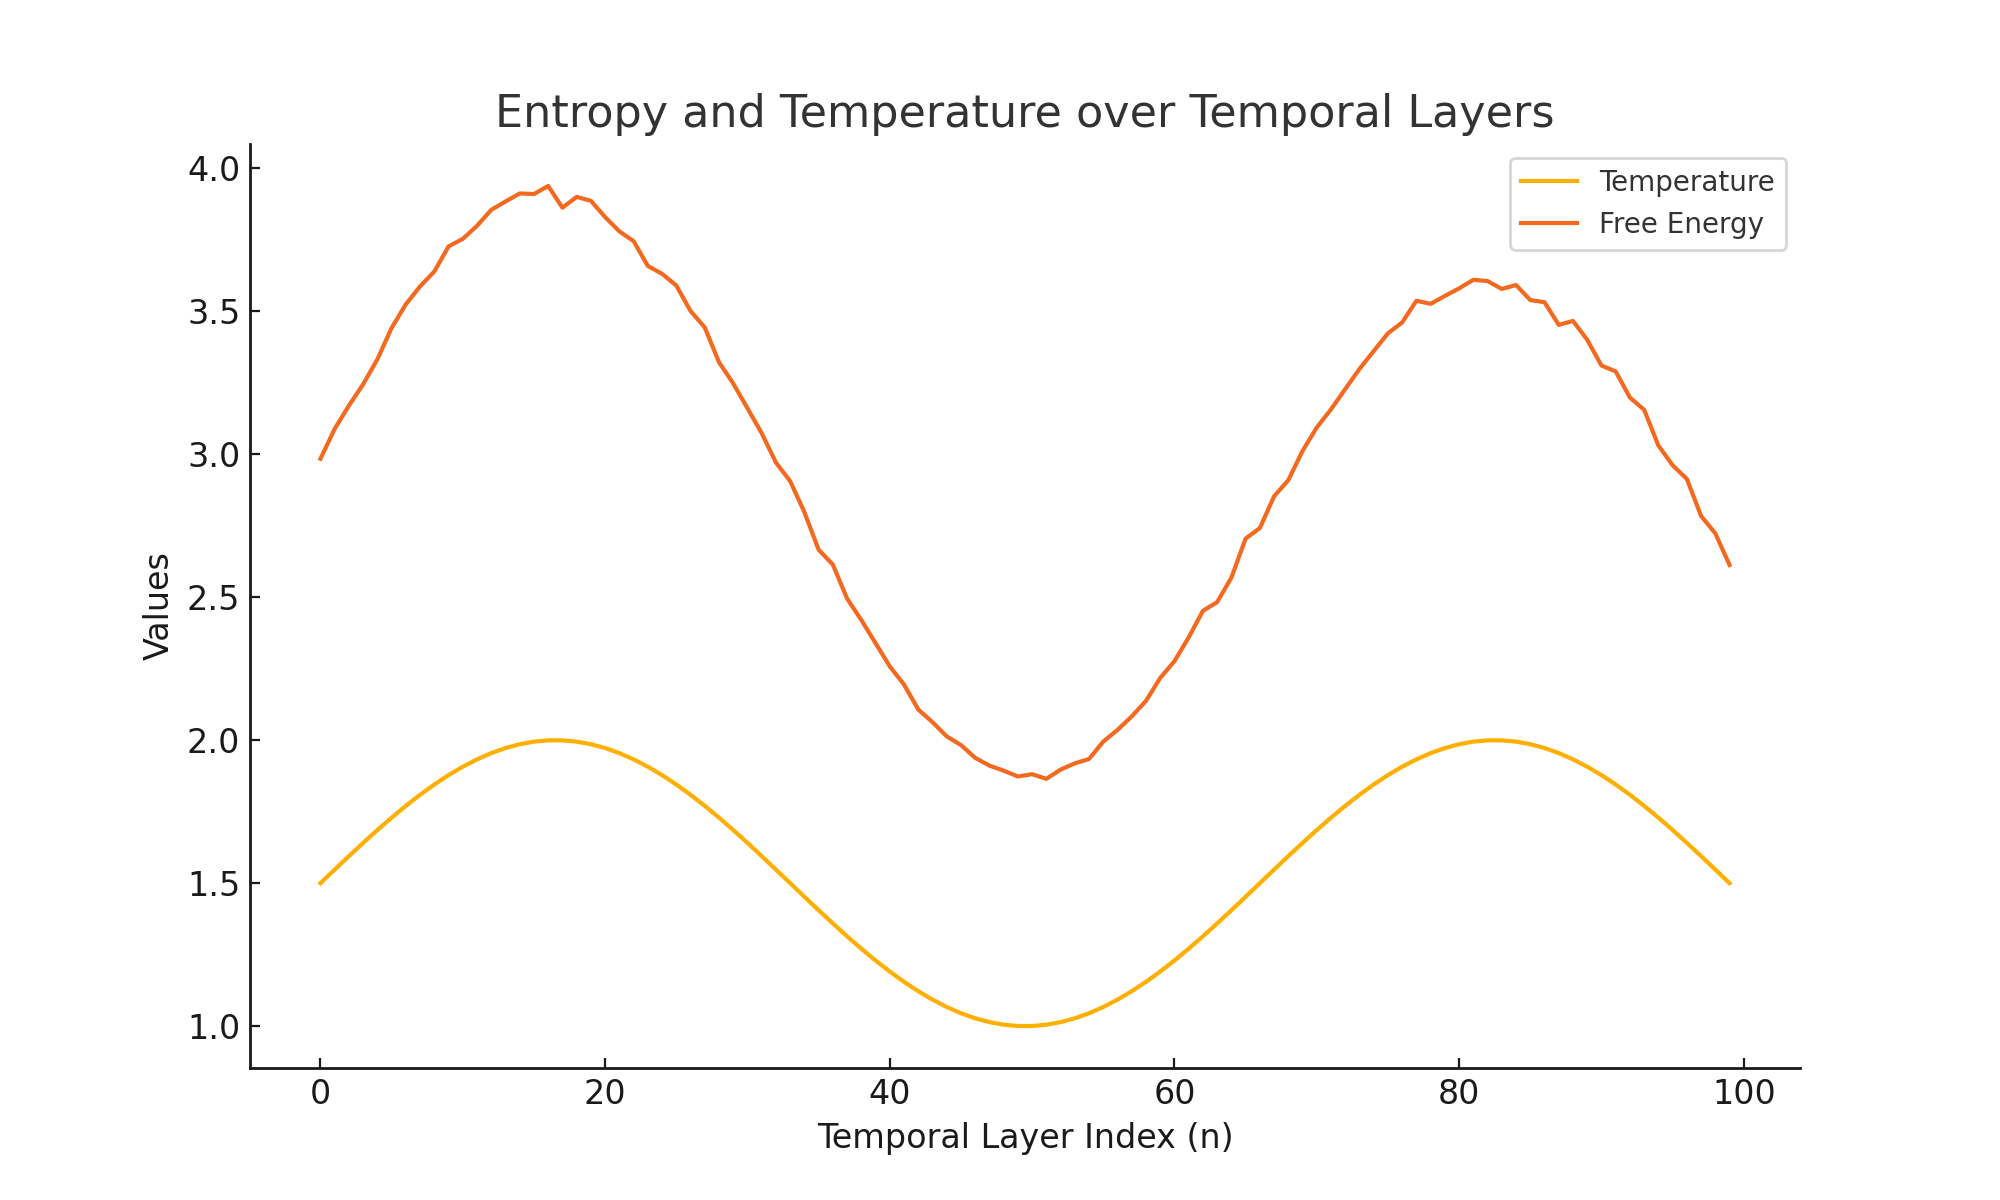
\includegraphics[width=0.9\linewidth]{05_Simulations/temp_free_energy.png}
\caption{Comparison of simulated temperature and free energy over time. Fluctuations are synthetic but reflect thermodynamic oscillations.}
\end{figure}

\begin{figure}[h!]
\centering
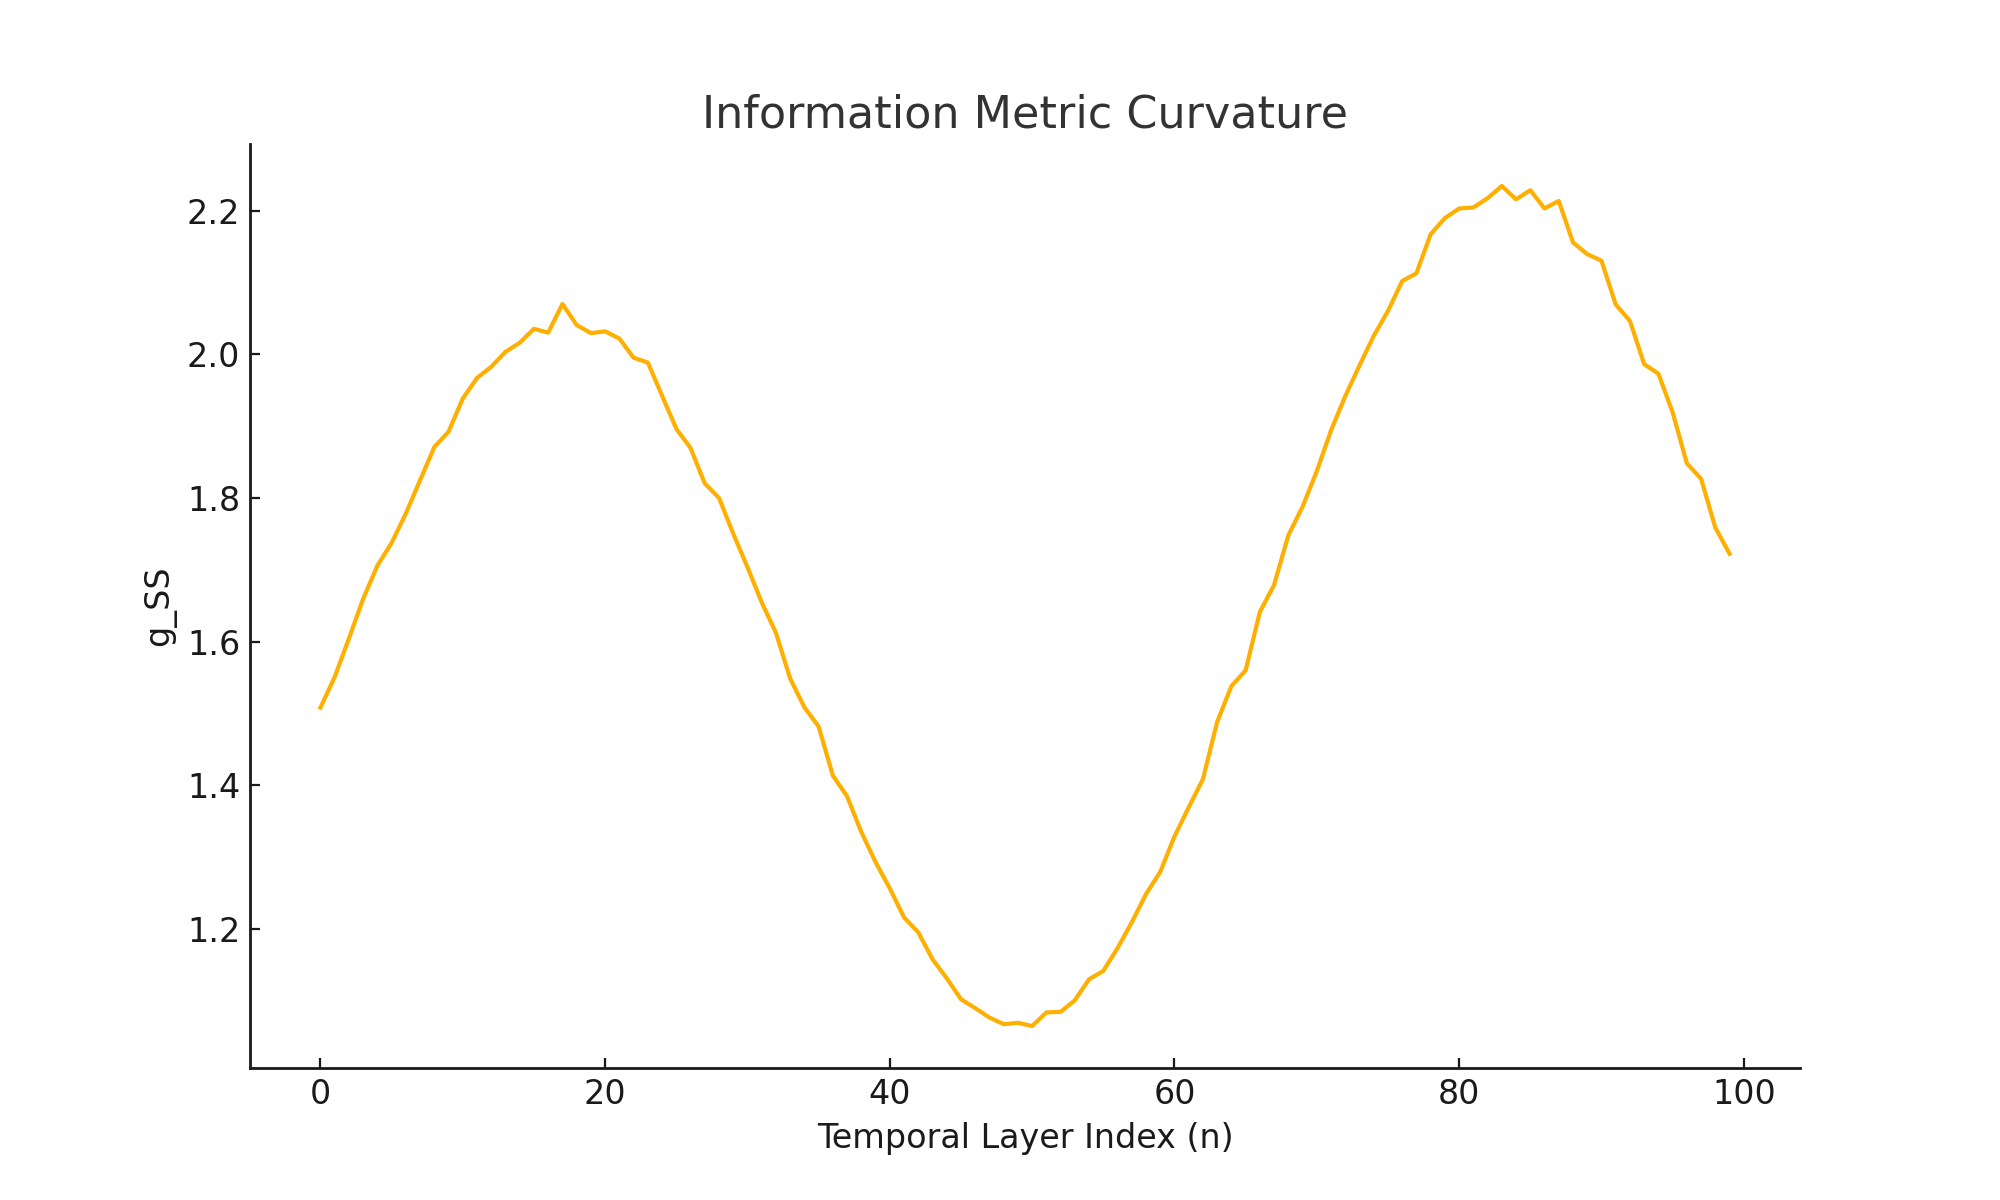
\includegraphics[width=0.9\linewidth]{05_Simulations/info_metric_curvature.png}
\caption{Information metric curvature $g_{SS}$ derived from synthetic entropy and temperature series.}
\end{figure}




\end{document}